%------------------------------  ------------------------------
%package list
\documentclass{article}
\usepackage[top=3cm, bottom=3cm, outer=3cm, inner=3cm]{geometry}
\usepackage{multicol}
\usepackage{graphicx}
\usepackage{url}
%\usepackage{cite}
\usepackage{hyperref}
\usepackage{array}
%\usepackage{multicol}
\newcolumntype{x}[1]{>{\centering\arraybackslash\hspace{0pt}}p{#1}}
\usepackage{natbib}
\usepackage{pdfpages}
\usepackage{multirow}
\usepackage[normalem]{ulem}
\useunder{\uline}{\ul}{}
\usepackage{svg}
\usepackage{xcolor}
\usepackage{listings}
\lstdefinestyle{ascii-tree}{
    literate={├}{|}1 {─}{--}1 {└}{+}1
  }
\lstset{basicstyle=\ttfamily,
  showstringspaces=false,
  commentstyle=\color{red},
  keywordstyle=\color{blue}
}
%\usepackage{booktabs}
\usepackage{caption}
\usepackage{subcaption}
\usepackage{float}
\usepackage{array}

\newcolumntype{M}[1]{>{\centering\arraybackslash}m{#1}}
\newcolumntype{N}{@{}m{0pt}@{}}

%------------------------------ ÍTEMS ------------------------------

\newcommand{\itemEmail}{hchoquehuancaz@unsa.edu.pe}
\newcommand{\itemStudent}{Hernan Andy Choquehuanca Zapana}
\newcommand{\itemCourse}{Fundamentos de la Programación II}
\newcommand{\itemCourseCode}{20232191}
\newcommand{\itemSemester}{II}
\newcommand{\itemUniversity}{Universidad Nacional de San Agustín de Arequipa}
\newcommand{\itemFaculty}{Facultad de Ingeniería de Producción y Servicios}
\newcommand{\itemDepartment}{Departamento Académico de Ingeniería de Sistemas e Informática}
\newcommand{\itemSchool}{Escuela Profesional de Ingeniería de Sistemas}
\newcommand{\itemAcademic}{2023 - B}
\newcommand{\itemInput}{Del 18 Septiembre 2023}
\newcommand{\itemOutput}{Al 20 Septiembre 2023}
\newcommand{\itemPracticeNumber}{02}
\newcommand{\itemTheme}{Arreglos Estándar}

%------------------------------  ------------------------------

\usepackage[english,spanish]{babel}
\usepackage[utf8]{inputenc}
\AtBeginDocument{\selectlanguage{Spanish}}
\renewcommand{\figurename}{Figura}
\renewcommand{\refname}{Referencias}
\renewcommand{\tablename}{Tabla} %esto no funciona cuando se usa babel
\AtBeginDocument{%
	\renewcommand\tablename{Tabla}
}

\usepackage{fancyhdr}
\pagestyle{fancy}
\fancyhf{}
\setlength{\headheight}{30pt}
\renewcommand{\headrulewidth}{1pt}
\renewcommand{\footrulewidth}{1pt}
\fancyhead[L]{\raisebox{-0.2\height}{
\includegraphics[width=3cm]{img/logo_episunsa.png}}}
\fancyhead[C]{\fontsize{7}{7}\selectfont	\itemUniversity \\ \itemFaculty \\ \itemDepartment \\ \itemSchool \\ \textbf{\itemCourse}}
\fancyhead[R]{\raisebox{-0.2\height}{
\includegraphics[width=1.2cm]{img/logo_abet}}}
\fancyfoot[L]{Estudiante Hernan Choquehuanca Zapana}
\fancyfoot[R]{\itemCourse}
\fancyfoot[C]{Página \thepage}

% para el codigo fuente
\usepackage{listings}
\usepackage{color, colortbl}
\definecolor{dkgreen}{rgb}{0,0.6,0}
\definecolor{gray}{rgb}{0.5,0.5,0.5}
\definecolor{mauve}{rgb}{0.58,0,0.82}
\definecolor{codebackground}{rgb}{0.95, 0.95, 0.92}
\definecolor{tablebackground}{rgb}{0.8, 0, 0}

\lstset{frame=tb,
	language=bash,
	aboveskip=3mm,
	belowskip=3mm,
	showstringspaces=false,
	columns=flexible,
	basicstyle={\small\ttfamily},
	numbers=none,
	numberstyle=\tiny\color{gray},
	keywordstyle=\color{blue},
	commentstyle=\color{dkgreen},
	stringstyle=\color{mauve},
	breaklines=true,
	breakatwhitespace=true,
	tabsize=3,
	backgroundcolor= \color{codebackground},
}

%------------------------------ INICIO DEL DOCUMENTO------------------------------

\begin{document}
	
	\vspace*{10px}
	
	\begin{center}	
		\fontsize{17}{17} \textbf{ Informe de Laboratorio \itemPracticeNumber}
	\end{center}
	\centerline{\textbf{\Large Tema: \itemTheme}}
	%\vspace*{0.5cm}	

	\begin{flushright}
		\begin{tabular}{|M{2.5cm}|N|}
			\hline 
			\rowcolor{tablebackground}
			\color{white} \textbf{Nota}  \\
			\hline 
			     \\[30pt]
			\hline 			
		\end{tabular}
	\end{flushright}	

	\begin{table}[H]
		\begin{tabular}{|x{4.7cm}|x{4.8cm}|x{4.8cm}|}
			\hline 
			\rowcolor{tablebackground}
			\color{white} \textbf{Estudiante} & \color{white}\textbf{Escuela}  & \color{white}\textbf{Asignatura}   \\
			\hline 
			{\itemStudent \par \itemEmail} & \itemSchool & {\itemCourse \par Semestre: \itemSemester \par Código: \itemCourseCode}     \\
			\hline 			
		\end{tabular}
	\end{table}		
	
	\begin{table}[H]
		\begin{tabular}{|x{4.7cm}|x{4.8cm}|x{4.8cm}|}
			\hline 
			\rowcolor{tablebackground}
			\color{white}\textbf{Laboratorio} & \color{white}\textbf{Tema}  & \color{white}\textbf{Duración}   \\
			\hline 
			\itemPracticeNumber & \itemTheme & 02 horas   \\
			\hline 
		\end{tabular}
	\end{table}
	
	\begin{table}[H]
		\begin{tabular}{|x{4.7cm}|x{4.8cm}|x{4.8cm}|}
			\hline 
			\rowcolor{tablebackground}
			\color{white}\textbf{Semestre académico} & \color{white}\textbf{Fecha de inicio}  & \color{white}\textbf{Fecha de entrega}   \\
			\hline 
			\itemAcademic & \itemInput &  \itemOutput  \\
			\hline 
		\end{tabular}
	\end{table}

%------------------------------ ACTIVIDADES (TAREA) ------------------------------

	\section{Tarea}
	\begin{itemize}		
		\item JUEGO DEL AHORCADO \\
        En este ejercicio se le solicita a usted implementar el juego del ahorcado utilizando el código parcial que se le entrega. \\
        Deberá considerar que:
        \begin{itemize}
            \item El juego valida el ingreso de letras solamente. En caso el usuario ingrese un carácter equivocado le dará el mensaje de error y volverá a solicitar el ingreso.
            \item El juego supone que el usuario no ingresa una letra ingresada previamente.
            \item El método ingreseLetra() debe ser modificado para incluir las consideraciones de validación.
            \item Puede crear métodos adicionales.
        \end{itemize}
        
		\item Utilizar Git para evidenciar su trabajo.

	\end{itemize}
		
	\section{Equipos, materiales y temas utilizados}
	\begin{itemize}
		\item Sistema Operativo Windows 11 Pro 22H2 64 bits.
		\item VIM 9.0.
		\item Visual Studio Code
		\item Git 2.41.1.
		\item Cuenta en GitHub con el correo institucional.
            \item Variables Simples
		\item Arreglos Estándar
        \item Métodos
	\end{itemize}
	
	\section{URL de Repositorio Github}
	\begin{itemize}
		\item URL del Repositorio GitHub para clonar o recuperar.
        \item \url{https://github.com/hernanchoquehuanca/fp2-23b.git}
		\item URL para el laboratorio 02 en el Repositorio GitHub.
		\item \url{https://github.com/hernanchoquehuanca/fp2-23b/tree/main/fase01/lab02}
	\end{itemize}
	
	\section{Actividades con el repositorio GitHub}
        
        
%-----------------------------------------------------------------------------------
%------------------------------------- ACTIVIDADES  --------------------------------
%-----------------------------------------------------------------------------------

% ACTIVIDAD 1
    \subsection{Commits}
    \subsubsection{Actividad 1 : Implementar el juego del ahorcado utilizando el código parcial que se entregó :}
    \begin{itemize}	
        \item Primero acomodamos y copiamos el código para luego empezar a completarlo
	\item El código fue el siguiente:
    \end{itemize}
    \lstinputlisting[language=Java, caption={Ejercicio01.java},numbers=left,]{src/Ejercicio01v1.java}
    
    \begin{lstlisting}[language=bash,caption={Commit: Copiando el código proporcionado y acomodandolo}][H]
		$ git add .
		$ git commit -m "Copiando el codigo proporcionado y acomodandolo"			
		$ git push -u origin main
	\end{lstlisting}


    \begin{itemize}	
        \item Para validar el ingreso de letras aceptadas se hizo uso de los códigos ASCII 
        \item Además para no usar dos condicionales que para mayúsculas y minúsculas, se usa el método "toUpperCase()" para validar el rango entre 65 y 90 
	\item El método fue el siguiente:
    \end{itemize}
    \lstinputlisting[language=Java, caption={Ejercicio01.java},numbers=left,]{src/Ejercicio01v2.java}

    \begin{lstlisting}[language=bash,caption={Commit: Completando el metodo ingreseLetra usando codigo ascii para validar las letras}][H]
		$ git add .
		$ git commit -m "Completando el metodo ingreseLetra usando codigo ascii para validar las letras"			
		$ git push -u origin main
    \end{lstlisting}
    
%%% 3
    
    \begin{itemize}	
        \item Para el método "letraEnPalabraSecreta" simplemente usaremos un bucle for que recorra por cada char de "palSecreta" con una condicional (if) que retorne true si en algun char coincide el ingresado por el jugador con el de la palabra.
        \item En caso de no haber coincidencias, al finalizar el bucle for se retornará falso.
    \end{itemize}

    \lstinputlisting[language=Java, caption={Ejercicio01.java},numbers=left,]{src/Ejercicio01v3.java}

    \begin{lstlisting}[language=bash,caption={Commit: Completando el metodo letraEnPalabraSecreta verificando char por char si hay una coincidencia}][H]
		$ git add .
		$ git commit -m "Completando el metodo letraEnPalabraSecreta verificando char por char si hay una coincidencia"			
		$ git push -u origin main
    \end{lstlisting}
    
%%% 4
    \begin{itemize}	
        \item En el método "mostrarBlancosActualizados" hubieron dos versiones con modificaciones.
        \item Primero, se intentó usar el método para retornar una variable que guarde las letras adivinadas anteriormente a la vez que los imprime, pero al momento de guardar la palabra sería tedioso, ya que guardaría un string donde cada letra tenga " " en medio. 
        \item Segundo, se creó un nuevo String para guardar los datos y mantener el String "blancos", luego lo retorna para que en las siguientes veces se muestre la palabra que ha ido completando con los anteriores aciertos.
    \end{itemize}

    \lstinputlisting[language=Java, caption={Ejercicio01.java},numbers=left,]{src/Ejercicio01v4.java}

    \begin{lstlisting}[language=bash,caption={Commit: Segunda version del metodo con cambios para mostrar las letras adivinadas previamente al jugador}][H]
		$ git add .
		$ git commit -m "Segunda version del metodo con cambios para mostrar las letras adivinadas previamente al jugador"			
		$ git push -u origin main
    \end{lstlisting}

    
%%% 5
    \begin{itemize}	
        \item Hubieron más modificaciones para que el String "blancos" pueda guardar el avance del jugador y a su vez nos sirva para el método "letraEnPalabraSecreta" 
        \item Además se modificó el método "mostrarBlancos" para que al crear el contenido del String "blancos" lo haga sin espacios en cada posición par
        \item Y la tercera modificación fue en el método "mostrarBlancosActualizados" ya que ahora que "blancos" no contiene espacios, se le agregarán sólo al momento de imprimirlos
        \\
        \item El código con todos los cambios mencionados anteriormente quedaría de la siguiente manera : 
    \end{itemize}

    \lstinputlisting[language=Java, caption={Ejercicio01.java},numbers=left,]{src/Ejercicio01v5.java}



%%% 6
    \begin{itemize}	
        \item A pesar de las modificaciones anteriores existían errores que aparecieron al momento de compilar.
        \item Primero, se agregó la condicional que determinaría si el jugador alcanzó el límite de intentos (6) o si completo la palabra secreta, esto usando break que terminará el bucle cuando se haya completado la palabra.
        \item Segundo, se implementó los mensajes al finalizar el juego, tanto si se ganase o perdiese.
        \item Tercero, se modificó el método "mostrarBlancos" ya que imprimía con saltos de línea, lo cual no era correcto visualmente.
        \item Cuarto, al momento de recibir la letra ingresada se aplicaba el toUpperCase() para que la letra quede modificada desde que se recibe.
        \item Finalmente para que el juego funcione correctamente se agregó el contador de intentos a la condicional que se ejecuta cuando el usuario no acierta la letra, de está manera sería posible ganar si la palabra secreta tiene más de 6 letras distintas
    \end{itemize}

    \newpage
    \begin{itemize}
        \item El código con todos los cambios ya mencionados es el siguiente: 
    \end{itemize}
	\lstinputlisting[language=Java, caption={Ejercicio01.java},numbers=left,]{src/Ejercicio01.java}
    \begin{figure}[H]
		\centering
		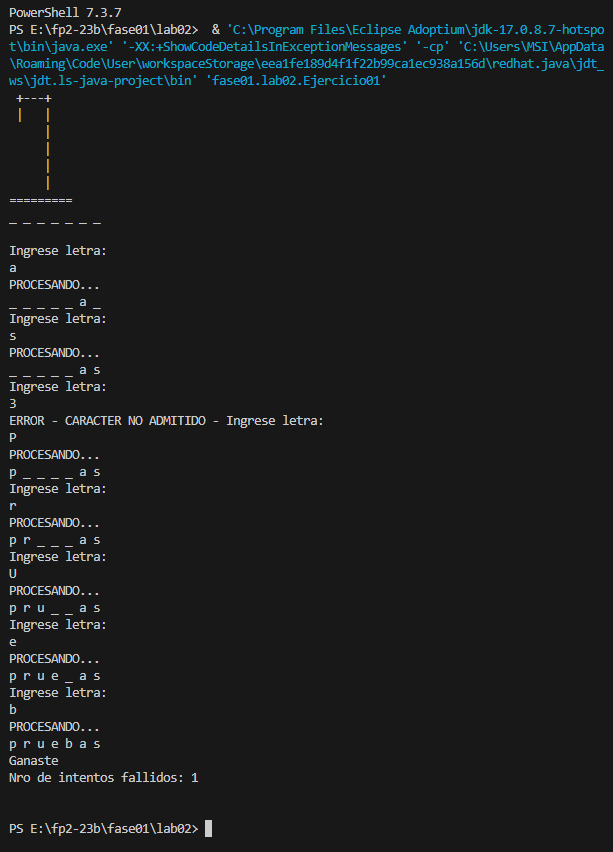
\includegraphics[width=0.8\textwidth,keepaspectratio]{img/prueba01.png}
		%\includesvg{img/automata.svg}
		%\label{img:mot2}
		%\caption{Product backlog.}
	\end{figure}
    
%-----------------------------------------------------------------------------------
%------------------------------ ESTRUCTURA DE LABORATORIO --------------------------
%-----------------------------------------------------------------------------------
    \newpage
	\subsection{Estructura de laboratorio 01}
	\begin{itemize}	
		\item El contenido que se entrega en este laboratorio es el siguiente:
	\end{itemize}
	
\begin{lstlisting}[style=ascii-tree]

lab01
|---|--- Ejercicio01.java
|--- latex
    |--- img
    |   |--- logo_abet.png
    |   |--- logo_episunsa.png
    |   |--- logo_unsa.jpg
    |   |--- prueba01.png
    |--- Informe_lab02.pdf
    |--- Informe_lab02.tex
    |--- src
        |---|--- Ejercicio01.java
        |---|--- Ejercicio01v1.java
        |---|--- Ejercicio01v2.java
        |---|--- Ejercicio01v3.java
        |---|--- Ejercicio01v4.java
        |---|--- Ejercicio01v5.java

\end{lstlisting}    

	\section{\textcolor{red}{Rúbricas}}
	
	\subsection{\textcolor{red}{Entregable Informe}}
	\begin{table}[H]
		\caption{Tipo de Informe}
		\setlength{\tabcolsep}{0.5em} % for the horizontal padding
		{\renewcommand{\arraystretch}{1.5}% for the vertical padding
		\begin{tabular}{|p{3cm}|p{12cm}|}
			\hline
			\multicolumn{2}{|c|}{\textbf{\textcolor{red}{Informe}}}  \\
			\hline 
			\textbf{\textcolor{red}{Latex}} & \textcolor{blue}{El informe está en formato PDF desde Latex,  con un formato limpio (buena presentación) y facil de leer.}   \\ 
			\hline 
			
			
		\end{tabular}
	}
	\end{table}
	
	\clearpage
%-----------------------------------------------------------------------------------
%------------------------------ RÚBRICA DE EVALUACIÓN ------------------------------
%-----------------------------------------------------------------------------------
 
	\subsection{\textcolor{red}{Rúbrica para el contenido del Informe y demostración}}
	\begin{itemize}			
		\item El alumno debe marcar o dejar en blanco en celdas de la columna \textbf{Checklist} si cumplio con el ítem correspondiente.
		\item Si un alumno supera la fecha de entrega,  su calificación será sobre la nota mínima aprobada, siempre y cuando cumpla con todos lo items.
		\item El alumno debe autocalificarse en la columna \textbf{Estudiante} de acuerdo a la siguiente tabla:
	
		\begin{table}[ht]
			\caption{Niveles de desempeño}
			\begin{center}
			\begin{tabular}{ccccc}
    			\hline
    			 & \multicolumn{4}{c}{Nivel}\\
    			\cline{1-5}
    			\textbf{Puntos} & Insatisfactorio 25\%& En Proceso 50\% & Satisfactorio 75\% & Sobresaliente 100\%\\
    			\textbf{2.0}&0.5&1.0&1.5&2.0\\
    			\textbf{4.0}&1.0&2.0&3.0&4.0\\
    		\hline
			\end{tabular}
		\end{center}
	\end{table}	
	
	\end{itemize}
	
	\begin{table}[H]
		\caption{Rúbrica para contenido del Informe y demostración}
		\setlength{\tabcolsep}{0.5em} % for the horizontal padding
		{\renewcommand{\arraystretch}{1.5}% for the vertical padding
		%\begin{center}
		\begin{tabular}{|p{2.7cm}|p{7cm}|x{1.3cm}|p{1.2cm}|p{1.5cm}|p{1.1cm}|}
			\hline
    		\multicolumn{2}{|c|}{Contenido y demostración} & Puntos & Checklist & Estudiante & Profesor\\
			\hline
			\textbf{1. GitHub} & Hay enlace URL activo del directorio para el  laboratorio hacia su repositorio GitHub con código fuente terminado y fácil de revisar. &2 &X &2 & \\ 
			\hline
			\textbf{2. Commits} &  Hay capturas de pantalla de los commits más importantes con sus explicaciones detalladas. (El profesor puede preguntar para refrendar calificación). &4 &X &3 & \\ 
			\hline 
			\textbf{3. Código fuente} &  Hay porciones de código fuente importantes con numeración y explicaciones detalladas de sus funciones. &2 &X &2 & \\ 
			\hline 
			\textbf{4. Ejecución} & Se incluyen ejecuciones/pruebas del código fuente  explicadas gradualmente. &2 &X &0.5 & \\ 
			\hline			
			\textbf{5. Pregunta} & Se responde con completitud a la pregunta formulada en la tarea.  (El profesor puede preguntar para refrendar calificación).  &2 &X &2 & \\ 
			\hline	
			\textbf{6. Fechas} & Las fechas de modificación del código fuente estan dentro de los plazos de fecha de entrega establecidos. &2 &X &2 & \\ 
			\hline 
			\textbf{7. Ortografía} & El documento no muestra errores ortográficos. &2 &X &2 & \\ 
			\hline 
			\textbf{8. Madurez} & El Informe muestra de manera general una evolución de la madurez del código fuente,  explicaciones puntuales pero precisas y un acabado impecable.   (El profesor puede preguntar para refrendar calificación).  &4 &X &3 & \\ 
			\hline
			\multicolumn{2}{|c|}{\textbf{Total}} &20 & &16.5 & \\ 
			\hline
		\end{tabular}
		%\end{center}
		%\label{tab:multicol}
		}
	\end{table}
	
\clearpage

%------------------------------ REFERENCIAS ------------------------------

\section{Referencias}
\begin{itemize}			
    \item \url{https://docs.oracle.com/javase/tutorial/java/nutsandbolts/variables.html}
    \item \url{https://docs.oracle.com/javase/8/docs/api/java/util/Arrays.html}
    \item \url{https://docs.oracle.com/javase/tutorial/java/javaOO/methods.html}
\end{itemize}	
	
%\clearpage
%\bibliographystyle{apalike}
%\bibliographystyle{IEEEtranN}
%\bibliography{bibliography}
			
\end{document}